\documentclass{article}

% General physics constructs
\newcommand{\bra}[1]{\langle #1 |}
\newcommand{\ket}[1]{| #1 \rangle }
\newcommand{\braket}[2]{\langle #1|#2\rangle}
\newcommand{\bbraket}[3]{ \langle #1 | #2 | #3 \rangle }
\newcommand{\norm}[1]{\| #1\|}
\newcommand{\avg}[1]{\left \langle #1 \right \rangle}
\newcommand{\angavg}[1]{\left \langle #1 \right \rangle}
\newcommand{\abs}[1]{\left \lvert #1 \right \rvert}
\newcommand{\VS}{\textit{\textbf{V}}}
\newcommand{\Tr}{\textrm{Tr}}
\renewcommand{\Re}{\textrm{Re}}
\renewcommand{\Im}{\textrm{Im}}
\newcommand{\basis}[1]{\{\ket{#1}\}}

\newcommand{\omegaqubit}{\omega_{10}}

% Figures. Example usage:
% \quickfig{\columnwidth}{my_image}{This is the caption}{fig:my_fig}
\DeclareRobustCommand{\quickfig}[4]{
\begin{figure}
\begin{centering}
\includegraphics[width=#1]{#2}
\par\end{centering}
\caption{#3}
\label{#4}
\end{figure}
}

\DeclareRobustCommand{\quickwidefig}[4]{
\begin{figure*}[h]
\begin{centering}
\includegraphics[width=#1]{#2}
\par\end{centering}
\caption{#3}
\label{#4}
\end{figure*}
}

%Packages
\usepackage{amsmath}
\usepackage{amstext}
\usepackage{amssymb}
\usepackage{appendix}
\usepackage{coseoul}
\usepackage{enumerate}
\usepackage{graphicx}
\usepackage{import}
\usepackage{lscape}
\usepackage{modular}

\usepackage[pdfpagemode=UseNone,pdfstartview=FitH,colorlinks=true,linkcolor=blue,citecolor=blue,urlcolor=blue]{hyperref}
\usepackage[all]{hypcap}



\title{Parametric Amplifier}
\author{Daniel Sank\\
\small{University of California Santa Barbara}\\
\small{presently Google Quantum AI}}
\date{18 March 2013}

\begin{document}

\maketitle

In this note we study the driven parametric oscillator.
This device can be use as an amplifier as will be shown at the end of the note.

\section{Equations of motion}

In this section we derive the equation of motion for a driven, damped Josephson oscillator with parametric modulation of its inductance.

\subsection{Josephson oscillator}

Consider a parallel resistor $R$, capacitor $C$, and Josephson junction of critical current $I_c$, driven by an external current source $I_s(t) = I_s \cos(\omega_s t + \theta)$.
The equation of motion for this circuit is
\begin{equation}
\ddot{\phi} + \frac{1}{RC}\dot{\phi} + \frac{1}{L_{J_0}C}\sin \phi = \frac{2\pi}{C \Phi_0} I_s \cos(\omega_s t + \theta)
\end{equation}
where $L_{J_0} \equiv \Phi_0 / 2\pi I_c$ is the un-biased inductance of the junction.
Defining $\omega_0 \equiv 1 / \sqrt{L_{J_0}C}$, $2 \Gamma \equiv 1/RC$, and $J \equiv  2\pi I_s / C \Phi_0$, we can re-write the equation of motion as
\begin{equation}
\ddot{\phi} + 2\Gamma \dot{\phi} + \omega_0^2 \sin \phi = J \cos(\omega_s t + \theta) .
\end{equation}

\subsection{Parametric pumping}

Suppose the junction were instead a DC SQUID. We could then modulate the inductance by driving flux through the SQUID loop. The inductance of the SQUID is then \begin{equation}
L(t) = L_{\textrm{dc}} + \Phi_p \frac{dL}{d\Phi}\cos(\omega_p t) \end{equation}
where $L_{\textrm{dc}}$ is the inductance of the SQUID under a constant flux bias, and $\Phi_p$ is the amplitude of the flux drive signal. This leads to a time dependent oscillation frequency \begin{eqnarray}
\omega_0(t) &=& (L_{\textrm{dc}}C)^{-1/2} \left(1 + \cos(\omega_p t) \frac{dL/L_{\textrm{dc}}} {d\Phi/\Phi_p} \right)^{-1/2} \\
&\approx& \omega_{0,\textrm{dc}} \left( 1 -\cos(\omega_p t) \frac{1}{2}\frac{dL/L_{\textrm{dc}}}{d\Phi/\Phi_p} \right) \\
&\equiv& \omega_{0,\textrm{dc}}\left( 1 - A\cos(\omega_p t) \right) \end{eqnarray}

Now the equation of motion is \begin{equation}
\ddot{\phi} + 2\Gamma \dot{\phi} + \omega_{0,\textrm{dc}}^2(1 - A \cos(\omega_p t))\sin(\phi) = J\cos(\omega_s t + \theta) \end{equation}
Taking only the linear term of the $\sin$ we get \begin{equation}
\ddot{\phi} + 2\Gamma \dot{\phi} + \omega_{0,\textrm{dc}}^2(1 - A \cos(\omega_p t))\phi = J\cos(\omega_s t + \theta) \label{eq:motion} \end{equation}
which is a driven, damped harmonic oscillator with time dependent frequency.

\section{Solution of equations of motion}

Equation (\ref{eq:motion}) is best studied in the frequency domain.
Making the transformation to frequency is easy using the following facts \begin{eqnarray}
\cos(\Omega t + \theta) &\rightarrow& \frac{1}{2}(2\pi)\left(e^{i \theta}\delta(\omega - \Omega) + e^{-i \theta} \delta(\omega + \Omega) \right) \nonumber \\
\phi(t)\cos(\Omega t) &\rightarrow& \frac{1}{2}\left( \tilde{\phi}(\omega-\Omega) + \tilde{\phi}(\omega+\Omega) \right) \nonumber \\
\dot{\phi}(t) &\rightarrow& i\omega \tilde{\phi}(\omega) \nonumber \end{eqnarray}
Using these equations and defining $L(\omega) \equiv (\omega_0^2 - \omega^2 +i2\omega\Gamma)$, we get \begin{equation}
\underbrace{L(\omega) \tilde{\phi}}_{\text{linear response}}
- \underbrace{\frac{1}{2} A \omega_0^2 \left[ \tilde{\phi}(\omega - \omega_p) + \tilde{\phi}(\omega + \omega_p) \right]}_{\text{modulated response}}
= \underbrace{\frac{1}{2}J(2\pi)\left[e^{i \theta}\delta(\omega-\omega_s) + e^{-i\theta}\delta(\omega+\omega_s) \right]}_{\text{source}} . \label{eq:eqOfMotionFrequency} \end{equation}

We want to find what $\tilde{\phi}(\omega)$ solves this equation.
If the parametric modulation were absent ($A=0$), then we would get the standard driven harmonic oscillator equation and $\phi$ would be a single tone at $\omega_s$.
However, the parametric drive produces frequency-shifted copies of $\tilde\phi$ so a single tone at $\omega_s$ does not work.

\begin{figure}
\begin{centering}
\includegraphics[width=12cm]{responseBalance.pdf} 
\par\end{centering}
\caption{The three terms in Eq. (\ref{eq:eqOfMotionFrequency}).
The source term is a pure tone at $\omega_s$.
The modulated response produces a copy of $\phi$ shifted by $\omega_p$.
a) Case where $\phi$ is a pure tone at $\omega_s$ with amplitude $\alpha$ (blue).
In this case, the linear and modulated response terms do not sum up to match the source.
b) Here $\phi$ includes another tone at $\omega_i$ with amplitude $\beta$ (red).
Now we can choose $\alpha$ and $\beta$ such that the linear and modulated responses sum to match the source.}
\label{Fig:responseBalance}
\end{figure}

To understand how to fix this, we construct a diagram representing the right and left hand sides of Eq. (\ref{eq:eqOfMotionFrequency}), as shown in Figure \ref{Fig:responseBalance}.
Figure \ref{Fig:responseBalance}\,a shows the frequency space representation of the source and response terms in Eq. \ref{eq:eqOfMotionFrequency}) assuming that $\tilde\phi$ were a single tone at $\omega_s$ with amplitude $\alpha$.
Adding the linear and modulated responses gives a shifted tone with amplitude $\alpha^*$ that has no counterpart in the source.
The only solution in this case is $\alpha=0$ which is trivial.
Now suppose the response has another tone at frequency $\omega_i$ with amplitude $\beta$ as shown by the red peaks in Figure \ref{Fig:responseBalance}\,b.
Now the frequency shifted copies can add both to match the source at $\omega_s$ and, if the amplitudes are chosen correctly, to cancel at $\omega_i$.
The response peak at $\omega_s$ is called the ``signal'' and the peak at $\omega_i$ is called the ``idler''.

Balancing the terms yields two equations: \begin{eqnarray}
L(\omega_s)\alpha - \frac{1}{2}A\omega_0^2 \beta^* &=& \frac{1}{2}J(2\pi)e^{i\phi} \\
L(\omega_i)\beta - \frac{1}{2}A\omega_0^2 \alpha^* &=& 0 . \end{eqnarray}
Solving the two simultaneous equations gives
\begin{equation}
\beta^* = - \frac{1}{2}A\omega_0^2 \frac{J'}{\left(\frac{1}{2}A\omega_0^2 \right)^2 + L(\omega_s)^2} \qquad
\alpha = L(\omega_s) \frac{J'}{\left(\frac{1}{2}A\omega_0^2 \right)^2 + L(\omega_s)^2} . \label{eq:alphabeta}
\end{equation}
In order to use the circuit as an amplifier we need gain.
From Eq. (\ref{eq:alphabeta}) we see that gain is achieved when
\begin{equation}
\left| \frac{1}{2}A\omega_0^2 + L(\omega_s)^2 \right| \ll 1 . \label{eq:gainCondition} \end{equation}
Equation (\ref{eq:gainCondition}) is satisfied when $L(\omega_s)$ is approximately purely imaginary, which occurs for $\omega_s \approx \omega_0$.
This makes sense, as we know the amplifier has large gain when the signal frequency is near the resonator mode center frequency.
%This also implies that $\alpha$ and $\beta$ are related by complex conjugation and an approximately 90 degree phase shift, which is the same as reflection about the line $\Im z = \Re z$.

\subsection{Drive at $\omega_i$}
If the drive is at the idler frequency the equations are \begin{eqnarray}
L(\omega_i)\beta - \frac{1}{2}A\omega_0^2 \alpha^* &=& \frac{1}{2}J(2\pi)e^{i\phi} \\
L(\omega_s)\alpha - \frac{1}{2}A\omega_0^2 \beta^* &=& 0 \end{eqnarray}
Solving gives \begin{eqnarray}
\beta^* &=& -\frac{1}{2}A\omega_0^2 \frac{J'}{\left( \frac{1}{2}A\omega_0^2 \right)^2 + L(\omega_s)^2} \\
\alpha &=& L(\omega_s) \frac{J'}{\left( \frac{1}{2}A\omega_0^2 \right)^2 + L(\omega_s)^2} \end{eqnarray}


\end{document}
